\documentclass[a4paper, 11pt]{article}

\usepackage[slovak]{babel}
\usepackage[utf8]{inputenc}
\usepackage[left=2cm, top=2.5cm, text={17cm, 28cm}]{geometry}
\usepackage{changepage}
\usepackage[unicode]{hyperref}
\usepackage{multirow}
\usepackage[ruled, linesnumbered, noline, longend]{algorithm2e}
\usepackage{graphics}
\usepackage{tikz}
\usepackage{pdflscape}
\usepackage{caption}

\def\Vdash{\mathop{\vdash}}

\begin{document}

\section*{Závislosť nehodovosti na triede komunikácie}

Táto správa sa zameriava na porovnanie nehodovosti podľa triedy komunikácie, na ktorej sa nehoda stala. Správa pracuje s nehodami, ktoré sa stali mimo obce, a na týchto typoch komunikácií:

\begin{itemize}
	\item diaľnice
	\item cesty 1. triedy
	\item cesty 2. triedy
	\item cesty 3. triedy.
\end{itemize}

Celkovo správa pracuje s údajmi o \textbf{223 622} nehodách. Graf na obrázku \ref{obr_1} zobrazuje všetky sledované dáta ako celkový počet nehôd, straty na životoch a zdraví, a hmotné škody, spôsobené na vozidlách.

\begin{figure}[h]
	\scalebox{0.63}{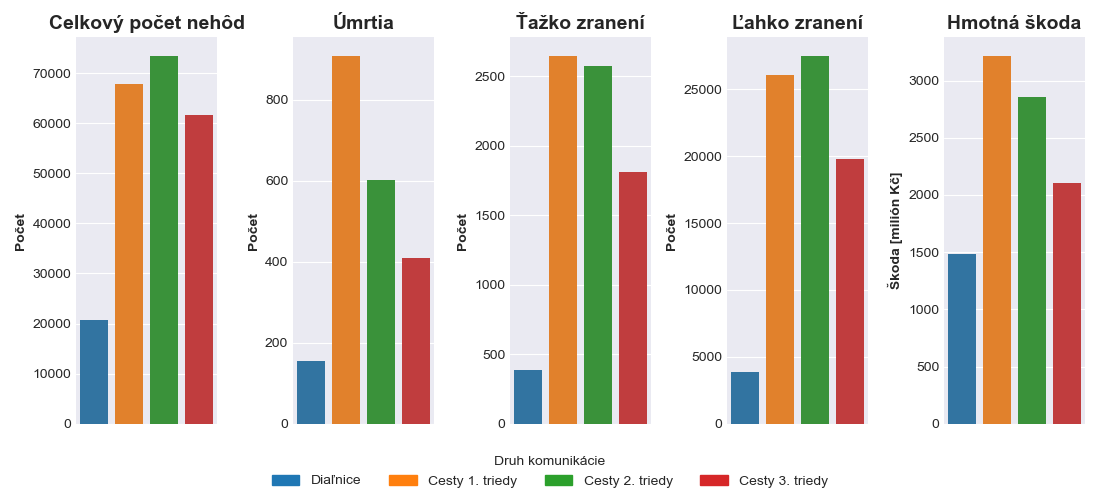
\includegraphics{fig.png}}
	\centering
	\caption{Prehľad sledovaných údajov}
	\label{obr_1}
\end{figure}

Najviac smrteľných nehôd sa stáva na cestách 1. triedy, v priemere zahynie \textbf{0.013} ľudí na 1 nehodu, napriek tomu, že najviac nehôd celkovo sa stáva na cestách 2. triedy. Naopak, najmenej nehôd celkovo ako aj smrteľných sa stáva na diaľniciach. V priemere zahynie \textbf{0.008} ľudí na 1 nehodu. Tabuľka \ref{tab_1} zobrazuje percentuálne zastúpenie podľa druhu komunikácie v jednotlivých ukazovateľoch.

\begin{center}
	\captionof{table}{Percentuálne zastúpenie v jednotlivých ukazovateľoch} 
	\begin{tabular}{lrrrrr}
	\hline
	                 & Počet nehôd   & Úmrtia   & Ťažko zranení   & Ľahko zranení   & Škoda [mil. Kč]   \\
	\hline
	 Diaľnice        & 9.25 \%        & 7.52 \%   & 5.19 \%          & 5.06 \%          & 15.39 \%           \\
	 Cesty 1. triedy & 30.31 \%       & 43.78 \%  & 35.68 \%         & 33.73 \%         & 33.27 \%           \\
	 Cesty 2. triedy & 32.84 \%       & 29.03 \%  & 34.72 \%         & 35.61 \%         & 29.58 \%           \\
 	Cesty 3. triedy & 27.59 \%       & 19.67 \%  & 24.42 \%         & 25.61 \%         & 21.77 \%           \\
	\hline
	\end{tabular}
	\label{tab_1}
\end{center}

Naopak, priemerná hmotná škoda spôsobená pri 1 nehode na diaľnici je \textbf{71 935.73 Kč} oproti priemernej hmotnej škode, spôsobenej pri 1 nehode na cestách 1. triedy, ktorá je \textbf{47 455.26 Kč}. Pričom nehody na diaľniciach tvoria \textbf{9.25 \%} a nehody na cestách 1. triedy \textbf{30.31 \%} z celkového počtu sledovaných nehôd.

\end{document}